\documentclass[12pt]{article}
\usepackage{graphicx}
\usepackage[margin = 1in]{geometry}
\usepackage{amsmath}
\usepackage{booktabs}
\usepackage{natbib}
\usepackage{lipsum}
\usepackage[colorlinks=true,citecolor=blue]{hyperref}

\title{Practicing LaTeX Paper}
\author{Sean Murphy\\
Statistics Major\\
University of Connecticut}

\begin{document}
\maketitle

\begin{abstract}
This is the abstract of my paper. 
\end{abstract}

\section{Introduction}
\label{sec:intro}

\lipsum[1]

\citet{larsen2005introduction} wrote an introductory text on mathematical statistics.  

\citep{weir2002estimating} wrote an article on estimating F statistics.  

% roadmap paragraph
This is how the rest of the paper will unfold. 
I will present the data in Section~\ref{sec:data}. 
I will provide an overview of the methods in Section~\ref{sec:math}. 
I will discuss the results in Section~\ref{sec:resu}. 
I will elaborate on the results with further discussion in Section~\ref{sec:disc}.

\section{Data}
\label{sec:data}

Here I will describe the data that was utilized in my research.  

The first equation that is pertinent to this analysis is:
\begin{equation}
    \label{eq:slope}
    y = mx + b
\end{equation}

Let us look at more closely at Equation~\eqref{eq:slope}.

In this equation, the expression $mx + b$ contains the slope, $m$, and the y-intercept, $b$.


\section{Methods}
\label{sec:math}

Here I will describe the methods that were used to analyze the data and draw conclusions

The second equation that is pertinent to this analysis is:
\begin{equation}
    \label{eq:int}
    \int_0^1x^2dx=\frac{1}{3}
\end{equation}

In Equation~\eqref{eq:int}, the integral of $x^2$ is $\frac{1}{3}x^3$, which, when evaluated from 0 to 1, yields $\frac{1}{3}$.

\section{Results}
\label{sec:resu}

Here I will summarize the results of the analysis.

\lipsum[3]

Table~\ref{tab:tabl} shows some of the findings from this analysis.

\begin{table}[tbp]
\caption{Here is the first table in this paper.}
\label{tab:tabl}
\centering
\begin{tabular}{rrr}
\toprule
x & y & z \\
\midrule
123 & 456 & 789 \\
012 & 345 & 678 \\
098 & 765 & 432 \\
\bottomrule
\end{tabular}
\end{table}

Figure~\ref{fig:figu} shows another important feature of the analysis.

\begin{figure}[tbp]
    \centering
    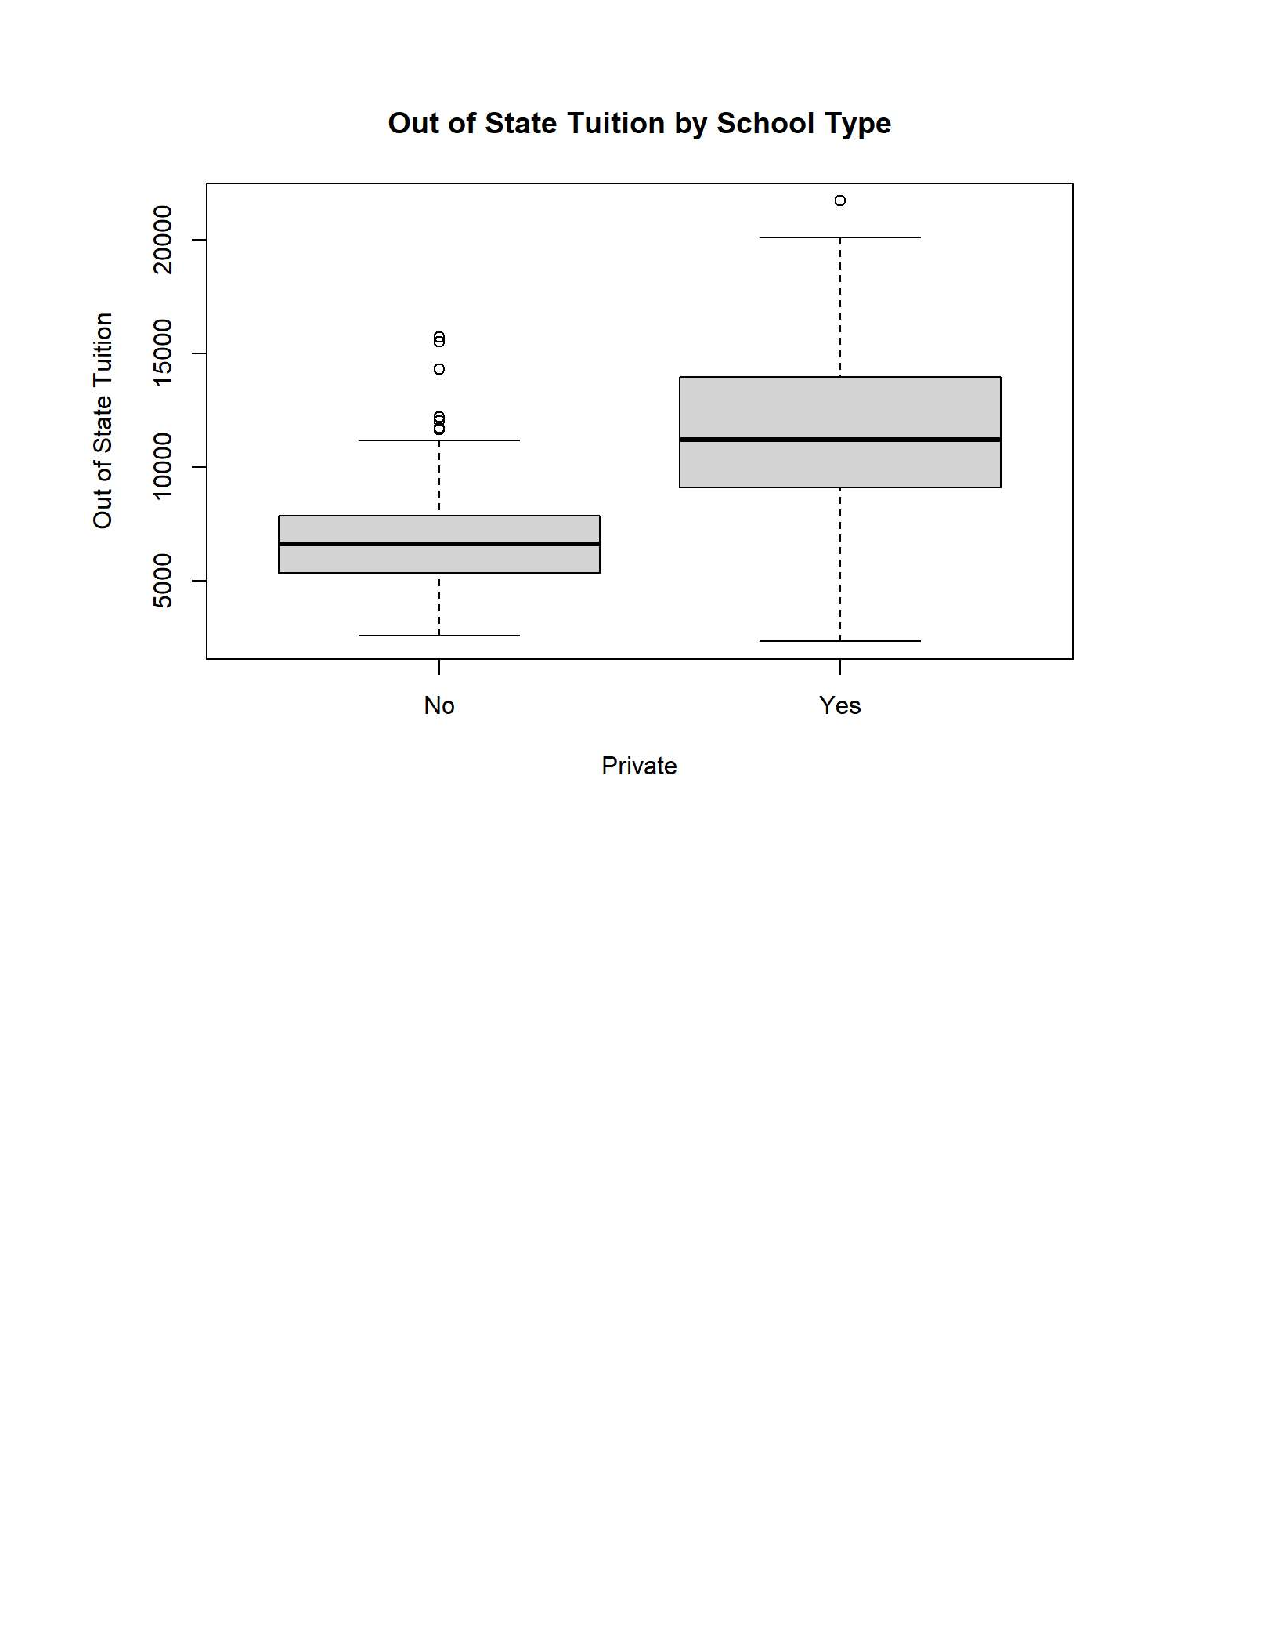
\includegraphics[width=\textwidth]{Practicing LaTeX Example Figure.pdf}
    \caption{This is the first figure in this paper.}
    \label{fig:figu}
\end{figure}

\section{Discussion}
\label{sec:disc}

Here I will reflect upon the impact of these results in the field. 

\lipsum[2]

\bibliography{PracitingLaTeXBibliography}

\end{document}
